\chapter{Approximation Schemes}
\label{chpt:app_schemes}
In this chapter we will introduce different approximation methods that we plan to use in our numerical simulations. We will go over equations governing their behavior and we also briefly mention some other approximations that were used in the past.

Parts of this chapter have been published in \textcite{2020MNRAS.493.2085V}.

\section{Motivation}
Various approximations in different scientific fields have always been studied in detail. Many non-linear equations cannot be solved analytically and one can hope to achieve at least some results using linearization or other perturbation theories of higher-order. Cosmological simulations are no exception. From the beginning of first attempts to simulate clustering of matter on large scales in the late '60s the approximate methods were developed to help understand the dynamics of the Universe. The greatest pioneering efforts to improve and validate these approximate methods have been undertaken in the '90s.

These analytic or semi-analytic methods can be used to understand the otherwise very complicated problem of structure formation. Instead of running a simulation ``blindly'' and trying to analyze them phenomenologically one can compare these simulations with much better understood approximate methods.

Besides the usefulness of approximations in getting an insight into gravitational evolution, they are very helpful in getting a large number of simulations quickly. In order to study BAO, one needs a high number of simulations with very large volume and a high number of particles which requires demanding resources. The BAO scale is of particular interest to us as it lies between the linear regime which can be studied analytically and the highly non-linear regime of halo formation which requires precise \nbodysim s. The semi-analytical methods are expected to work very well in this regime.

In this chapter, we describe several approximations that have been studied in the past -- Zel'dovich approximation and its \textit{truncated} extension, frozen-flow approximation, and frozen-potential approximation. The Zel'dovich approximation has been studied extensively in the past and here we use it mainly as a reference for comparison in the context of the other approximations.

\section{Recapitulation of the linear theory}
Here we remind some results of the linear theory previously presented in \autoref{chpt:cosmo_evol}. We rewrite the equations using variables more suited for cosmological simulations. We will be working in comoving coordinates -- the comoving position $\mb x$ is defined in terms of the proper position coordinate $\mb r = a\mb x$. The comoving velocity $\mb v$ is then defined as a derivative with respect to cosmic time $t$, $\mb v = \dot{\mb x}$, where the overdot denotes a time derivative. Particles move in the Newtonian gravitational potential, $\Phi$. The equations for linear perturbations then read
\eq{
	\label{eq:lin_per_a}
	\dot\delta + \nabla\cdot\mb v &= 0, \\
	\label{eq:lin_per_b}
    \dot{\mb v} + 2\frac{\dot a}{a} \mb v &= -\frac{1}{a^2}\nabla\Phi, \\
\begin{split}
	\label{eq:lin_per_c}
	\Delta\Phi &= 4\pi G\bar\rho a^2 \delta \\
    			&= \frac32 H_0^2\Omega_{m, 0}\frac\delta a \equiv \mu^{-1}\frac\delta a\,,
\end{split}
}
where we defined the constant $\mu\equiv\left(\frac32 H_0^2\Omega_{m, 0}\right)^{-1}$. In this linear regime, the time and space dependence of the overdensity evolution are separable and we can write $\delta(a, \mb x)=D(a)\delta_0(\mb x)$ where the growth factor $D$ represents the growing solution (we neglect the decaying mode) and is normalized to unity at the present time.

It is often useful to rewrite these equations with a different time variable, namely the scale factor $a$. This is convenient both from the numerical and theoretical points of view because the quantities are ``more constant''. With the new time-variable $a$ and comoving velocity $\mb u = \dd \mb x/\dd a$, equation \eqref{eq:lin_per_a} becomes
\eq{
\label{eq:continuity_a}
	\dddd D a \delta_0 + \nabla\cdot\mb u = 0\,,
}
where $\dd D/\dd a = 1$ in the Einstein--de Sitter universe (hereafter EdS) and so the divergence of the velocity field remains constant in both time and space. Equation \eqref{eq:lin_per_b} then becomes
\seq{
	\label{eq:motion_EdS}
	\dddd{\mb u}{a} &= -\frac{3}{2a}\left[\mb u + \mu\nabla\Phi \right] \\
\intertext{in EdS and, more generally,}
	\label{eq:motion_LCDM}
	\dddd{\mb u}{a} &= -\frac{3}{2a}\left[\mb u\left(1+\Omega_\Lambda\right) + \mu\nabla\Phi\left(1-\Omega_\Lambda\right)\right]
}
in the \LCDM\ universe. The omega factor of the cosmological constant
\eq{
	\Omega_\Lambda(a) = \frac{\Omega_{\Lambda,0}a^3}{\Omega_{m,0} + \Omega_{\Lambda,0}a^3}
}
rises from $0$ to $\Omega_{\Lambda,0}$ and becomes significant $(>5\%)$ around redshift $z\approx2.5$. The transformation \eqref{eins_trans} from the Jordan frame to the Einstein frame introduces non-standard coupling of the chameleon field to standard matter resulting in the fifth force \eqref{cham_force}. Using our new variables, this equation reads
\eq{
	\label{eq:cham_force}
	\dddd{\mb u_{\chi}}{a} = -\frac{3\mu}{2a}\frac{\beta}{\Mpl}\mb{\nabla}\chi \,.
}
Equation \eqref{eq:lin_per_c} expressed with the growth factor reads
\eq{
\label{eq:poisson_a}
	\Delta\Phi(\mb x, a) = \mu^{-1}\frac D a \delta_0(\mb x)\,.
}
%%%%%%%%%%%%%%%%%%%%%%%%%%%%%%%%%%%%%%%%
% Zel'dovich Approximation
%%%%%%%%%%%%%%%%%%%%%%%%%%%%%%%%%%%%%%%%
\section{Zel'dovich approximation}
The Zel'dovich approximation \parencite[hereafter ZA;][]{1970A&A.....5...84Z} bears its name after a pioneer in the study of large-scale structure, a Soviet physicist Yakov Zel'dovich. The ZA provides an intuitive way to understand the emergence of filamentary structures (cosmic web) and can realize the model of non-linear structure formation even though it is based only on linear approximations \parencite{2014MNRAS.439.3630W}. The Zel’dovich approximation predicts the rich structure of voids, clusters, sheets, and filaments observed in the Universe.

The ZA is based on an ansatz that particles move in straight lines in the Lagrangian frame
\eq{
\label{eq:ZA}
	\mb x(\mb q, a) = \mb q + D(a)\mb S(\mb q)\,,
}
where $\mb q$ are the initial positions (Eulerian coordinates) of a particle and $\mb S$ is some displacement field. Inserting equation \eqref{eq:ZA} into the continuity equation \eqref{eq:continuity_a} yields
\eq{
	-\nabla\cdot S = \delta_0\,.
}
Combining with the Poisson equation \eqref{eq:poisson_a}, we can see that \eqref{eq:ZA} represents a potential flow, $\mb S = -\nabla\phi_V$, where the velocity potential $\phi_V$ obeys the Poisson equation
\eq{
	\label{eq:poisson_vel}
	\Delta\phi_V = \delta_0
}
and has a simple relation to the gravitational potential
\eq{
	\label{eq:vel_new}
	\phi_V=\mu\frac a D \Phi\,.
}
This results to ZA being
\eq{
	\mb x(\mb q, a) = \mb q - D(a)\mb\nabla \phi_V(\mb q)\,.
}
Note that the velocity potential is not exactly a potential of our velocity field $\mb u$ but
\eq{
	\label{eq:ZA_u}
	\mb u\ZA(\mb x) = -\dddd D a \nabla\phi_V(\mb q)\,.
}
The ZA differs from other approximations (among other things) in how this (constant) velocity potential, $\phi_V$, enters the equations of motion. To avoid having different definitions of the \textit{real} velocity potential for the velocity fields in each approximation, we take the equation \eqref{eq:poisson_vel} as defining the velocity potential $\phi_V$.

The deformation tensor is defined as
\eq{
	d_{ij}=\partpart{x_i}{q_j}=\delta_{ij}+D\partpart{\nabla_i\phi_V}{q_j}\,.
}
The eigenvectors of the deformation tensor determine the principal directions of the collapse and the corresponding eigenvalues determine the time when the compression will be infinite. The density is given through eigenvalues $\lambda_i$ as
\eq{
	\rho=\frac{\bar\rho}{(1-D\lambda_1)(1-D\lambda_2)(1-D\lambda_3)}\,.
}
The time when the density in ZA becomes infinite corresponds to particles crossing the paths of other particles. Once this shell-crossing has occurred, the approximation has formally broken down, since there are no forces present to slow down the particles and capture them within halos.

In \autoref{fig:slice_dens_ZA} we show a comparison of the simulations with ZA at four different redshifts through the projected density field. At redshift $z=\ztwo$ the cosmic web still looks nice but after that, at redshifts $z=\zthree, \zfour$, we can see that shell-crossing occurred and the overall picture gets blurry. The large-scale structures remain visible but the small-scale structures get diluted at later times.
\begin{figure*}[!htbp]
	\begin{adjustwidth}{-1cm}{-1cm}
	\centering
		\begin{subfigure}{0.5\linewidth}
			\includegraphics[width=1.0\linewidth]{{simulations_approx/dens/za_dens_512m_1p_1024M_200b_z\zone}.png}
			\caption{$z=\zone$}
		\end{subfigure}%
		\begin{subfigure}{0.5\linewidth}
			\includegraphics[width=1.0\linewidth]{{simulations_approx/dens/za_dens_512m_1p_1024M_200b_z\ztwo}.png}
			\caption{$z=\ztwo$}
		\end{subfigure}
		\begin{subfigure}{0.5\linewidth}
			\includegraphics[width=1.0\linewidth]{{simulations_approx/dens/za_dens_512m_1p_1024M_200b_z\zthree}.png}
			\caption{$z=\zthree$}
		\end{subfigure}%
		\begin{subfigure}{0.5\linewidth}
			\includegraphics[width=1.0\linewidth]{{simulations_approx/dens/za_dens_512m_1p_1024M_200b_z\zfour}.png}
			\caption{$z=\zfour$}
		\end{subfigure}
	\end{adjustwidth}
		\caption{Projected density field at different redshifts for the Zel'dovich approximation. Each slice has a box-length of $200~\Mpch$ and is $1~\Mpch$ thick.}
		\label{fig:slice_dens_ZA}
\end{figure*}
%%%%%%%%%%%%%%%%%%%%%%%%%%%%%%%%%%%%%%%%
% Truncated Zel'dovich Approximation
%%%%%%%%%%%%%%%%%%%%%%%%%%%%%%%%%%%%%%%%
\section{Truncated Zel'dovich approximation}
The shell-crossing and diffusion of particles on small scales in ZA happens the sooner the more power there is on small scales. \textcite{1993MNRAS.260..765C} suggested an improvement of the ZA by removing power on these small non-linear scales, i.e. to set the initial power spectrum to zero for wave-numbers $k$ greater than a non-linear scale $k_{nl}$ defined as
\eq{
\label{eq:k_nl}
    \frac{a^2(t)}{2\pi^2}\int_0^{k_{nl}}P(k)\dd k=1\,,
}
where the power spectrum $P(k)$ was defined in \eqref{eq:pk} as
\eq{
  \label{eq:pk_cp}
  P(k)(2\pi)^3\delta_{\rm D}(k-k')\equiv \left\langle \hat\delta(k)\hat\delta^*(k')\right\rangle\,.
}

\textcite{doi:10.1093/mnras/269.3.626} further improved this truncation by applying a Gaussian window instead of an abrupt cutoff
\eq{
W(k)=e^{-k^2/2k^2_{G}}\,,
}
where the smoothing scale $k_{G}$ is 1 to 1.5 times $k_{nl}$. This filtering leads to the so-called truncated Zel'dovich approximation (TZA). This removes most of the strongly non-linear behavior and allows the Zel’dovich pancakes to be seen.

In \autoref{fig:slice_dens_TZA} we show a comparison of the simulations with TZA at four different redshifts through the projected density field. We see clear differences in comparison with ZA. Large-scale structures evolve similarly to ZA but we see clear artifacts on small scales given by artificial cutoff at these scales. These small-scale structures in filaments are not so diluted as in the case of ZA, however, a lot of particles remain in voids where they are frozen due to the lack of the initial kick.

\begin{figure*}[!htbp]
	\begin{adjustwidth}{-1cm}{-1cm}
	\centering
		\begin{subfigure}{0.5\linewidth}
			\includegraphics[width=1.0\linewidth]{{simulations_approx/dens/tza_dens_512m_1p_1024M_200b_z\zone}.png}
			\caption{$z=\zone$}
		\end{subfigure}%
		\begin{subfigure}{0.5\linewidth}
			\includegraphics[width=1.0\linewidth]{{simulations_approx/dens/tza_dens_512m_1p_1024M_200b_z\ztwo}.png}
			\caption{$z=\ztwo$}
		\end{subfigure}
		\begin{subfigure}{0.5\linewidth}
			\includegraphics[width=1.0\linewidth]{{simulations_approx/dens/tza_dens_512m_1p_1024M_200b_z\zthree}.png}
			\caption{$z=\zthree$}
		\end{subfigure}%
		\begin{subfigure}{0.5\linewidth}
			\includegraphics[width=1.0\linewidth]{{simulations_approx/dens/tza_dens_512m_1p_1024M_200b_z\zfour}.png}
			\caption{$z=\zfour$}
		\end{subfigure}
	\end{adjustwidth}
		\caption{Projected density field at different redshifts for the truncated Zel'dovich approximation. Each slice has a box-length of $200~\Mpch$ and is $1~\Mpch$ thick.}
		\label{fig:slice_dens_TZA}
\end{figure*}
%%%%%%%%%%%%%%%%%%%%%%%%%%%%%%%%%%%%%%%%
% Frozen-flow Approximation
%%%%%%%%%%%%%%%%%%%%%%%%%%%%%%%%%%%%%%%%
\section{Frozen flow approximation}
The frozen-flow, or frozen-field, approximation (FFA) was originally proposed by \textcite{Matarrese:1992be} as the exact solution of equation \eqref{eq:motion_EdS} in EdS
\eq{
  \label{eq:FFA_orig}
  \tilde{\mb u}\FFA(\mb x) = \mb u_0(\mb x) = -\mu\nabla\Phi(\mb x) = -\nabla\phi_V(\mb x)\,.
}
The velocity field $\tilde{\mb u}$ is frozen at each point to its initial value, i.e.
\eq{
	\partpart{\tilde{\mb u}}{a} = 0\,.
}
These equations are very similar to ZA but now the particles update their velocities to the local value of the velocity field (not the initial value), without any memory of their previous motion. This can be viewed as a movement of particles under some force in a medium with very large viscosity. In our case of cosmological simulations, gravity represents the attractive force while Hubble friction represents the informal equivalent of a ``damping'' or ``viscous'' force.

Originally, \textcite{Matarrese:1992be} stated three main reasons of why should the FFA work:
\begin{itemize}
\item FFA is, by construction, consistent with linear theory and follows correctly the evolution at early times. Keeping the linear approximation for the velocity potential is justified by the fact that this quantity is more sensitive to large wavelength modes than the density, and is, therefore, less affected by strongly non-linear evolution.
\item Stream-lines are frozen to their initial shape, so multistream regions cannot form and FFA avoids the formation of caustics at a finite time and can, therefore, work well after shell-crossing would occur in ZA. A particle moving according to FFA has zero velocity at minima (or maxima) of the gravitational potential. It will slow down its motion when approaching such a position -- particles in FFA would need infinite time to reach such places. Particles move along curved paths and once they come close to pancake configurations they curve their trajectories, moving almost parallel to them, trying to reach the positions of filaments.
\item This type of dynamics implies an artificial thickening of particles around pancakes, filaments, and knots, which mimics the real gravitational clustering around these types of structures.
\end{itemize}

The definition \eqref{eq:FFA_orig} is, however, no longer valid in the general \LCDM\ cosmology where even in the linear regime both gravitational potential and velocity field undergo evolution. We generalize FFA for the \LCDM\ cosmology by adding an extra time dependence in equation \eqref{eq:FFA_orig}
\eq{
	\label{eq:FFA}
	\mb u\FFA(\mb x, a) = -\dddd D a(a)\nabla\phi_V(\mb x)\,.
}
This velocity field solves \eqref{eq:motion_LCDM} exactly, due to the definition of the growth factor and its relation to the velocity field in the linear regime (see equation \eqref{eq:continuity_a}).

Although equation \eqref{eq:FFA} now does not represent a \textit{frozen} flow, particles still move along the same characteristic curves as in EdS, just with different velocities. The particle trajectories are described by the integral equation
\eq{
	\label{eq:FFA_int}
	\mb x(a) = \mb q + \int_0^a\dd \tilde a\mb u\FFA(\mb x(\tilde a), \tilde a)\,.
}

In \autoref{fig:slice_dens_FFA} we show a comparison of the simulations with FFA at four different redshifts through the projected density field. Unlike in the case of ZA or TZA there is no shell-crossing and structures remain clear even at later times. As the particles approach minima of the gravitational potential, they slow down and we can see that resulting structures are elongated along stream-lines.
\begin{figure*}[!htbp]
	\begin{adjustwidth}{-1cm}{-1cm}
	\centering
		\begin{subfigure}{0.5\linewidth}
			\includegraphics[width=1.0\linewidth]{{simulations_approx/dens/ff_dens_512m_1p_1024M_200b_z\zone}.png}
			\caption{$z=\zone$}
		\end{subfigure}%
		\begin{subfigure}{0.5\linewidth}
			\includegraphics[width=1.0\linewidth]{{simulations_approx/dens/ff_dens_512m_1p_1024M_200b_z\ztwo}.png}
			\caption{$z=\ztwo$}
		\end{subfigure}
		\begin{subfigure}{0.5\linewidth}
			\includegraphics[width=1.0\linewidth]{{simulations_approx/dens/ff_dens_512m_1p_1024M_200b_z\zthree}.png}
			\caption{$z=\zthree$}
		\end{subfigure}%
		\begin{subfigure}{0.5\linewidth}
			\includegraphics[width=1.0\linewidth]{{simulations_approx/dens/ff_dens_512m_1p_1024M_200b_z\zfour}.png}
			\caption{$z=\zfour$}
		\end{subfigure}
	\end{adjustwidth}
		\caption{Projected density field at different redshifts for the frozen flow approximation. Each slice has a box-length of $200~\Mpch$ and is $1~\Mpch$ thick.}
		\label{fig:slice_dens_FFA}
\end{figure*}
%%%%%%%%%%%%%%%%%%%%%%%%%%%%%%%%%%%%%%%%
% Frozen-potential Approximation
%%%%%%%%%%%%%%%%%%%%%%%%%%%%%%%%%%%%%%%%
\section{Frozen potential approximation}
The frozen-potential approximation (FPA) was introduced by \textcite{1994MNRAS.266..227B}. They exploit the fact that the gravitational potential changes much more slowly than the density contrast, and hence may be viewed as essentially frozen. Moreover, like the velocity potential in FFA is more sensitive to large wavelength modes, this is doubly true for gravitational potential. They solved equation \eqref{eq:motion_EdS} at each time-step with the initial (constant) gravitational potential. In \LCDM
\eq{
	\label{eq:FPA}
	\dddd{\mb u\FPA}{a} &= -\frac{3}{2a}\left[\mb u\FPA(\mb x,a)\left(1+\Omega_\Lambda(a)\right) + \frac D a \nabla\phi_V(\mb x)\left(1-\Omega_\Lambda(a)\right)\right]
}
and the particle trajectories are given as in the case of FFA\,
\eq{
	\mb x(a) = \mb q + \int_0^a\dd \tilde a\mb u\FPA(\mb x(\tilde a), \tilde a)~.
}
Particles now follow the linear \textit{gravitational} potential (which evolves slightly in \LCDM) instead of the initial \textit{velocity} potential as in the case of FFA. Equation \eqref{eq:FPA} drives the particle velocities (approximately) to the velocities of FFA but unlike in the FFA, particles now keep their inertia. Same as in the case of FFA, the particles tend to move along the pancakes towards regions of lower potential to end up in a few clumps. The acceleration used in FPA is largest in regions where the instantaneous velocity vector points along the gradient of the potential, as happen for particles after they cross the pancake. In FFA the inertia of particles is ignored, whereas in the Zel'dovich approximation inertia is assumed to dominate over the change in the force field. FPA takes into consideration both factors but assumes a constant potential.

In \autoref{fig:slice_dens_FPA} we show a comparison of the simulations with FPA at four different redshifts through the projected density field. At the first sight, it looks similarly as in the case of FFA, especially at early times. For $z=\zthree, \zfour$ we can see the differences due to the fact that particles have an inertia and resulting structures are not so elongated as in the case of FFA.
\begin{figure*}[!htbp]
	\begin{adjustwidth}{-1cm}{-1cm}
	\centering
		\begin{subfigure}{0.5\linewidth}
			\includegraphics[width=1.0\linewidth]{{simulations_approx/dens/fp_dens_512m_1p_1024M_200b_z\zone}.png}
			\caption{$z=\zone$}
		\end{subfigure}%
		\begin{subfigure}{0.5\linewidth}
			\includegraphics[width=1.0\linewidth]{{simulations_approx/dens/fp_dens_512m_1p_1024M_200b_z\ztwo}.png}
			\caption{$z=\ztwo$}
		\end{subfigure}
		\begin{subfigure}{0.5\linewidth}
			\includegraphics[width=1.0\linewidth]{{simulations_approx/dens/fp_dens_512m_1p_1024M_200b_z\zthree}.png}
			\caption{$z=\zthree$}
		\end{subfigure}%
		\begin{subfigure}{0.5\linewidth}
			\includegraphics[width=1.0\linewidth]{{simulations_approx/dens/fp_dens_512m_1p_1024M_200b_z\zfour}.png}
			\caption{$z=\zfour$}
		\end{subfigure}
	\end{adjustwidth}
		\caption{Projected density field at different redshifts for the frozen potential approximation. Each slice has a box-length of $200~\Mpch$ and is $1~\Mpch$ thick.}
		\label{fig:slice_dens_FPA}
\end{figure*}

%%%%%%%%%%%%%%%%%%%%%%%%%%%%%%%%%%%%%%%%
% Particle-mesh simulation
%%%%%%%%%%%%%%%%%%%%%%%%%%%%%%%%%%%%%%%%
\section{Particle-mesh simulation}
For comparison with other approximations, we also implemented the particle-mesh code, i.e. a simulation where the gravitation potential evolves according to the current position of particles but the particles feel only this long-range force without any short-range forces (for details see \autoref{sec:PM}). The particles move according to the equation of motion \eqref{eq:motion_LCDM} and the gravitational potential evolve according to Poisson equation \eqref{eq:lin_per_c}.

In \autoref{fig:slice_dens_all} we show a comparison of all approximation methods with PM at $z=0$ through the projected density field. Here we can see side-by-side the main differences between individual approximation methods: ZA with diluted small-scale structures, TZA with (almost) frozen small-scale structures, FFA and FPA with elongated structures. We see that PM simulation has more concentrated filaments but also more particles in voids than ZA, FFA, and FPA.
% \afterpage{%
\begin{figure*}[!htbp]
	\thisfloatpagestyle{empty}
	\begin{adjustwidth}{-2cm}{-2cm}
	\centering
		\begin{subfigure}{0.4\linewidth}
			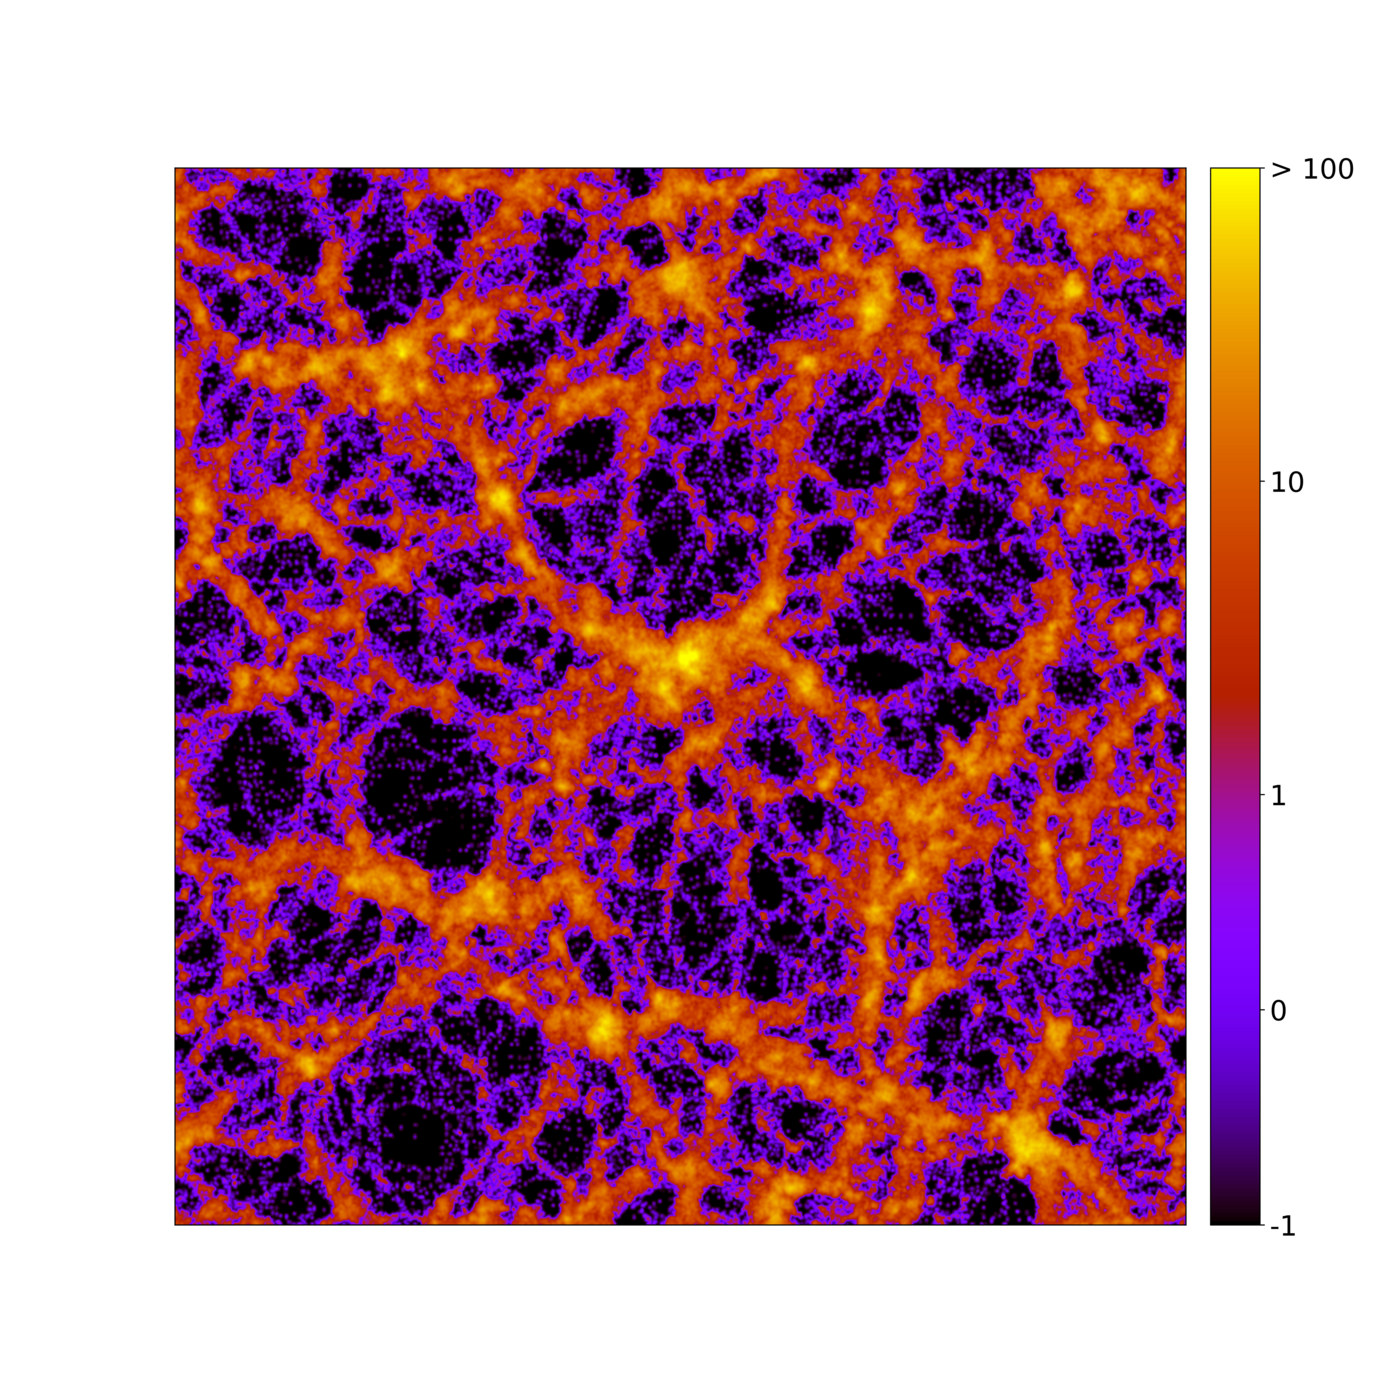
\includegraphics[width=1.0\linewidth]{{simulations_approx/dens/za_dens_512m_1p_1024M_200b_z0.00}.png}
			\caption{Zel'dovich approximation}
		\end{subfigure}%
		\begin{subfigure}{0.4\linewidth}
			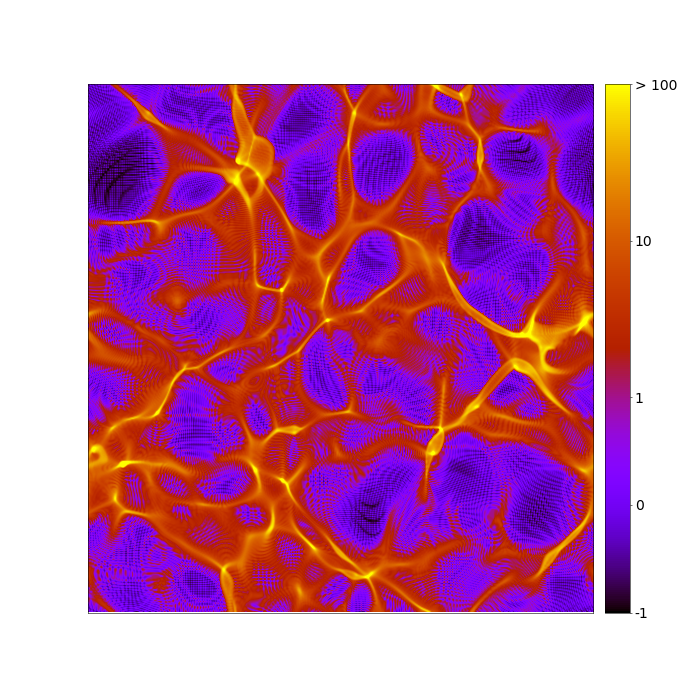
\includegraphics[width=1.0\linewidth]{{simulations_approx/dens/tza_dens_512m_1p_1024M_200b_z0.00}.png}
			\caption{Truncated Zel'dovich approximation}
		\end{subfigure}
		\begin{subfigure}{0.4\linewidth}
			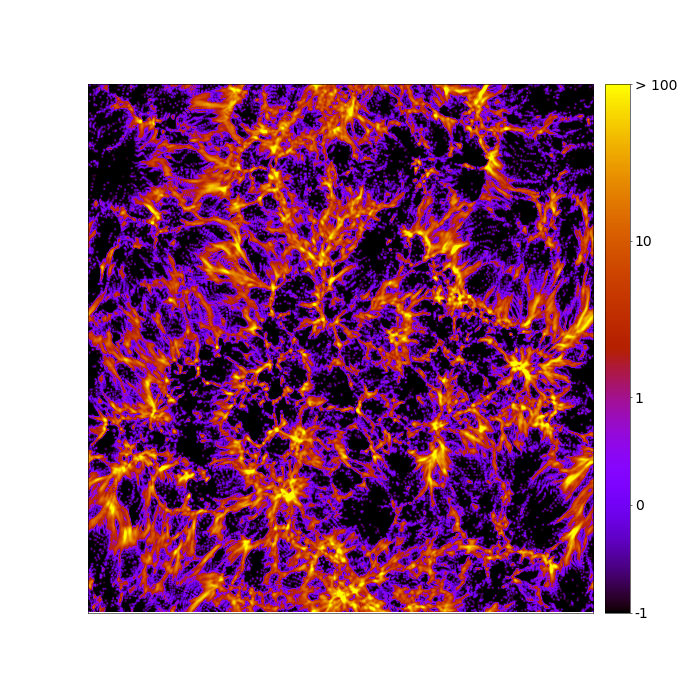
\includegraphics[width=1.0\linewidth]{{simulations_approx/dens/ff_dens_512m_1p_1024M_200b_z0.00}.png}
			\caption{Frozen-flow approximation}
		\end{subfigure}%
		\begin{subfigure}{0.4\linewidth}
			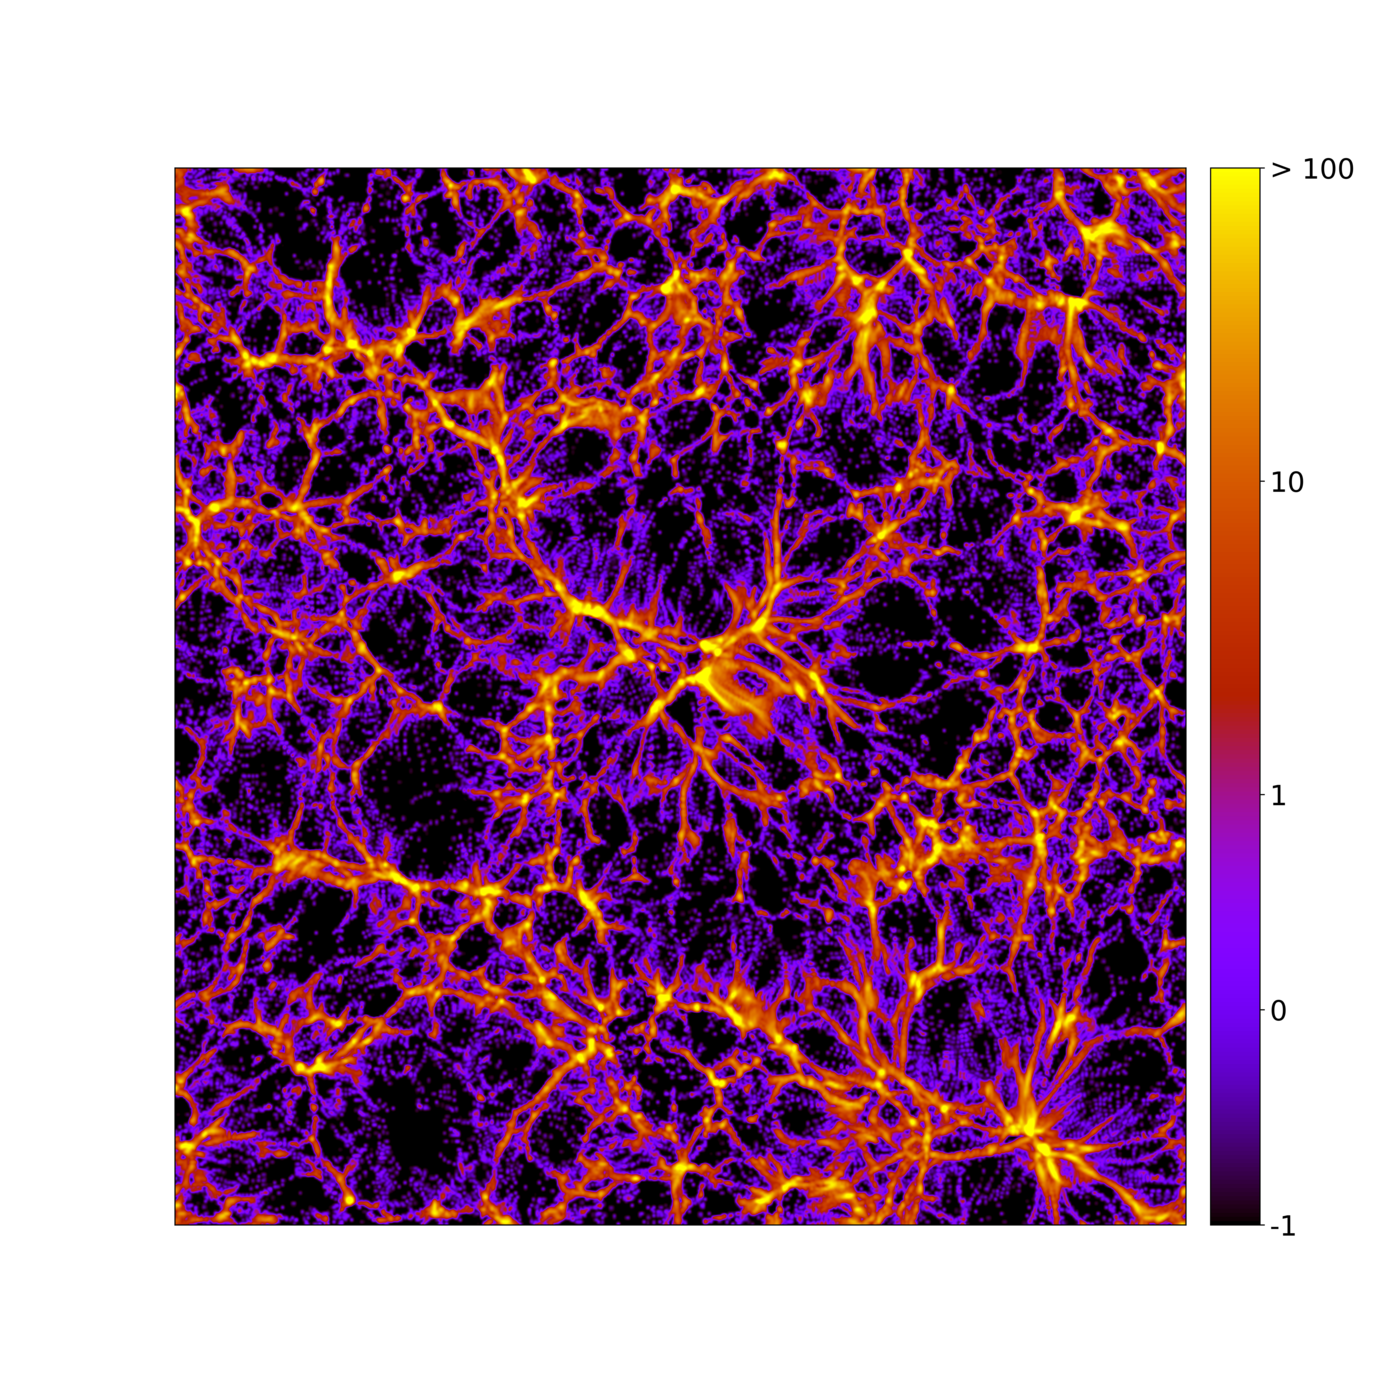
\includegraphics[width=1.0\linewidth]{{simulations_approx/dens/fp_dens_512m_1p_1024M_200b_z0.00}.png}
			\caption{Frozen-potential approximation}
		\end{subfigure}
		\begin{subfigure}{0.4\linewidth}
			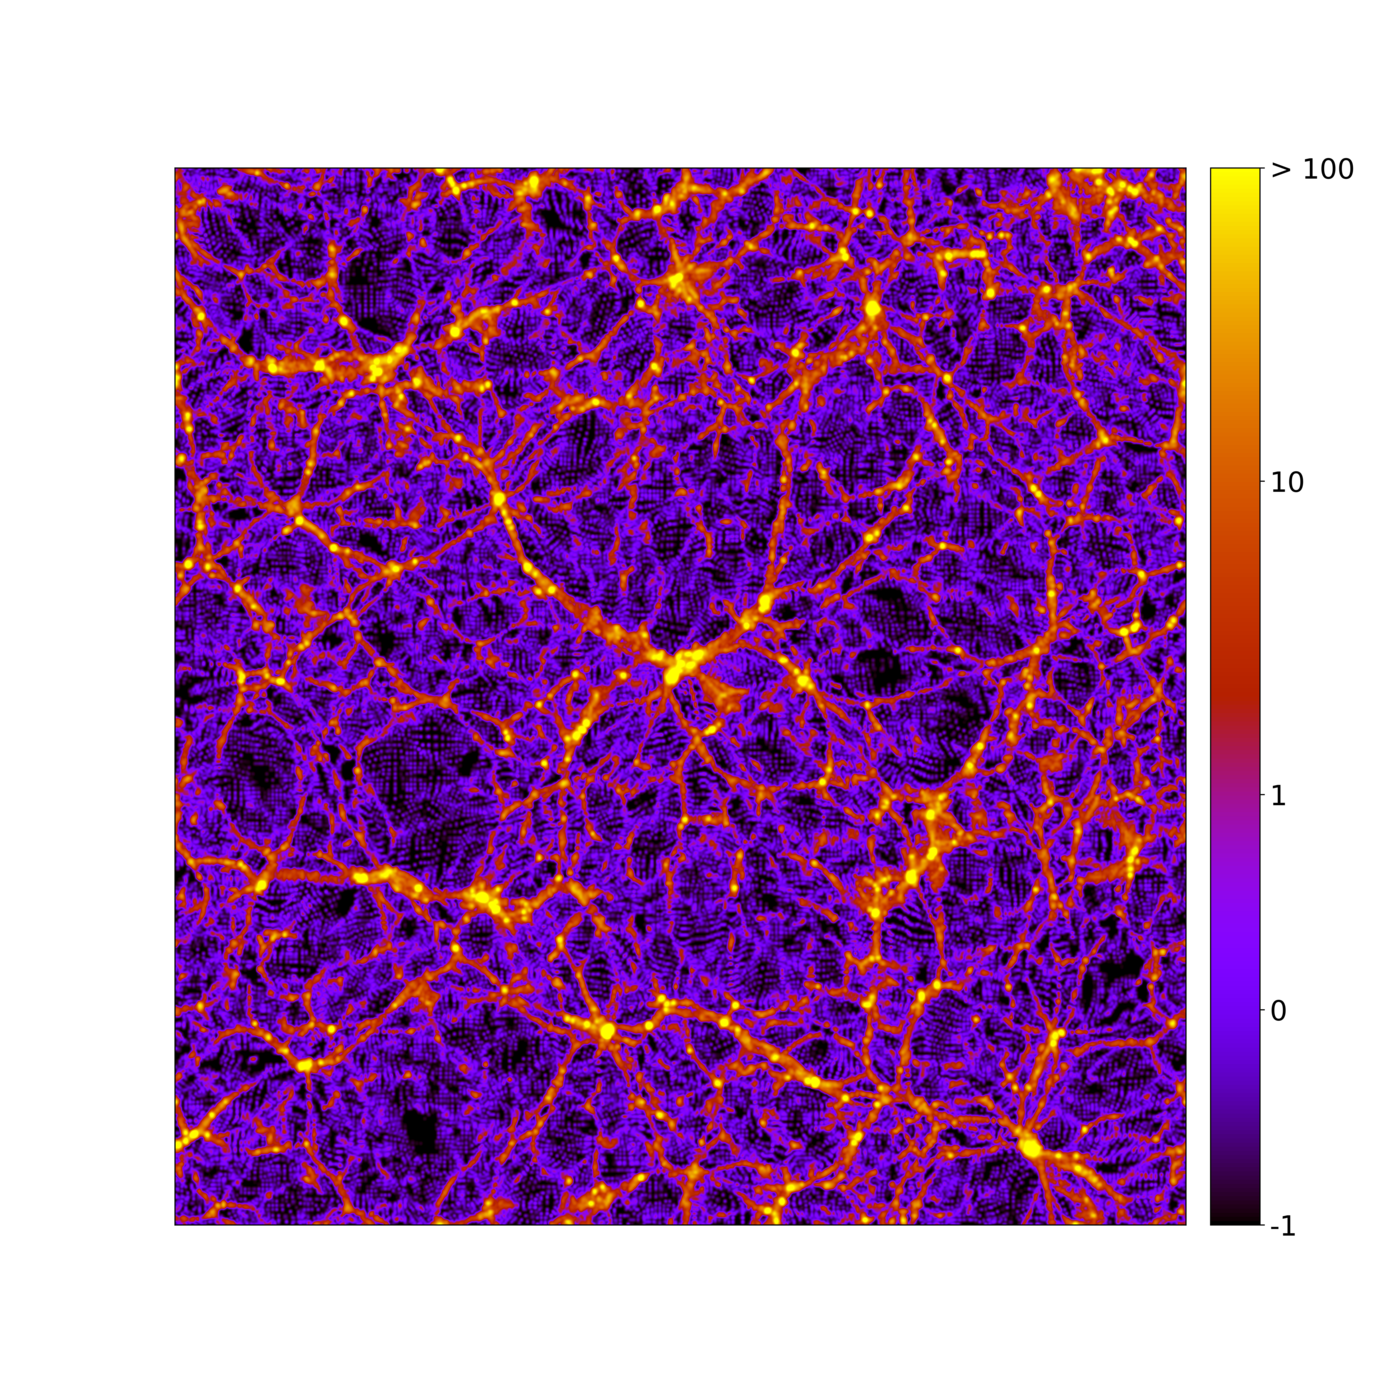
\includegraphics[width=1.0\linewidth]{{simulations_approx/dens/pm_dens_512m_1p_1024M_200b_z0.00}.png}
			\caption{PM simulation}
		\end{subfigure}
	\end{adjustwidth}
		\caption{Projected density field at redshift $z=0$ for the different approximations, all run with the same initial conditions. Each slice has a box-length of $200~\Mpch$ and is $1~\Mpch$ thick.}
		\label{fig:slice_dens_all}
\end{figure*}
\floatpagestyle{plain}
% } %% end afterpage


%%%%%%%%%%%%%%%%%%%%%%%%%%%%%%%%%%%%%%%%
% Approximation methods in modified gravity
%%%%%%%%%%%%%%%%%%%%%%%%%%%%%%%%%%%%%%%%
\section{Approximation methods in modified gravity}
Here we remind the basic chameleon equations we want to solve numerically. The non-linear Poisson equation
\eq{
\label{eq:cham_u_cp}
	\Delta\left(\chi/\chi_a\right)= C_\chi(a)\left[1+\delta-\left(\frac{\chi_a}{\chi}\right)^{1-n}\right]\,,
}
where
\eq{
	C_\chi(a)\equiv\frac{3H_0^2\Omega_m}{2\Phiscrz}a^{-3\frac{2-n}{1-n}}=\left(a\mu\Phiscra\right)^{-1}\,,
}
the linear solution
\eq{
\label{eq:chi_lin_x_cp}
	\chi(\mb x, a) = \chi_a(a)\left(1 + \frac{\Phi_G(\mb x, a)}{\Phiscra(a)} \right)\,.
}
the linear solution in $k-$space
\eq
{
\label{eq:chi_lin_k_cp}
	\hat{\chi}(k)=-\frac{\chi_a}{1-n}\frac{m^2}{m^2+k^2}\hat{\delta}(k) = -\frac{\beta\bar\rho_m}{\Mpl}\frac{\hat{\delta}(k)}{k^2+m^2}\,.
}
where the mass of the chameleon field is
\eq{
    \label{eq:chi_m_cp}
	m^2(a)\equiv\frac{1-n}{a\mu\Phiscra}\,,
}
and the screened solution inside massive objects
\eq{
	\chi=\frac{\chi_a}{\left(1+\delta\right)^{1/(1-n)}}\,.
	\label{eq:chi_bulk_cp}
}

When applying the approximation methods to the chameleon equations, we have three choices on how to arrive at an approximate solution:
\begin{enumerate}
\item \label{itm:lin_q} Purely linear prediction in $(\mb q, a)$-space, solution \eqref{eq:chi_lin_x_cp}

\item \label{itm:lin_k} Purely linear prediction in $(\mb k, a)$-space, solution \eqref{eq:chi_lin_k_cp}

\item \label{itm:nl_x} Non-linear prediction in $(\mb x, a)$-space, solution \eqref{eq:cham_u_cp}
\end{enumerate}

Choice \ref{itm:lin_q} means that there is no computational overhead and we can simply take the chameleon force to be $2\beta^2a^{-2}$ of the gravitational one. This method clearly overestimates the chameleon force at early times when the chameleon's Compton wavelength is short. This is because the solution \eqref{eq:chi_lin_x_cp} does not take into account the non-zero mass of the field.

A better choice is to use \ref{itm:lin_k} where the non-zero mass is incorporated. This solution adds relatively little computational overhead over normal gravity -- needing (at least) one Fourier transform and also extra storage. The overdensity $\delta(\mb k, a)$ is either the linearly evolved one, i.e. $\delta(\mb k, a) = D(a)\delta_0(\mb k)$, or we can compute $\delta$ at each time-step from the current positions of particles. This adds extra computation when assigning the mass of particles on the grid and one extra Fourier transform to get $\delta(\mb k, a)$. 
However, we cannot use \eqref{eq:chi_lin_k_cp} blindly to get a solution in real space as this linear approximation breaks down inside massive objects where we would get a negative solution. This effect is similar to usage of linear evolution for $\delta$ where we can end up with regions where $\delta<-1$. We need to check if the resulting chameleon field is positive and fix it where it is not. We use the screening regime value \eqref{eq:chi_bulk_cp} to get a positive solution. We will refer to this prediction as pseudo-linear since it can address some effects of the screening mechanism.

The most expensive choice is \ref{itm:nl_x} where we must iteratively solve nonlinear equations. Unlike other methods, this one can address the screening regime inside and near massive objects but at the cost of the most computational overhead.

%%%%%%%%%%%%%%%%%%%%%%%%%%%%%%%%%%%%%%%%
% Other approximations
%%%%%%%%%%%%%%%%%%%%%%%%%%%%%%%%%%%%%%%%
\section{Other approximations}
Approximations described previously are studied numerically in detail in the next chapter. Here we present a few of the other approximations studied in the past or used today.

\subsection{Adhesion approximation}
The adhesion approximation was introduced in \textcite{1989MNRAS.236..385G}. To study the evolution of density inhomogeneities they used the model of non-linear diffusion (Burger`s equation), that gives an approximate description of the growth of structures at the advanced non-linear stage of gravitational instability.

To overcome problems of ZA with shell-crossing they propose a solution of ``sticking articles.'' Particles move according to ZA until they ran into one another. Then they move together, with the velocity conserving momentum. This model can be described mathematically by inserting the viscous term into equations of motion, simulating attractive forces of gravity
\eq{
	\dddd{\mb u\AAP}{a}=\nu\partpart{^2\mb u}{\mb x^2}\,.
}
The Burger`s equation has an analytical solution that can be used to study the formation of structures. For more information regarding the adhesion approximation see  also \textcite{1990MNRAS.247..260W,1994ApJ...428...28M}.

\subsection{Stable clustering}
It was proposed by \textcite{1974ApJ...189L..51P} that clustering in the very non-linear regime might be understood by assuming that regions of high-density contrast undergo virialization and subsequently maintain a fixed proper density, hence stable clustering. The correlation function for a population of such systems would then simply evolve according to
\eq{
	\xi(r,a)\propto1/\bar\rho\propto a^3\,.
}
\textcite{1991ApJ...374L...1H} developed a method for interpolating between linear theory on large scales and the non-linear predictions of the stable clustering hypothesis on small scales. They showed that the non-linear volume-averaged two-point correlation function could be parameterized by a simple function of the linear correlation function
\eq{
	\bar\xi_{NL}=f(\bar\xi_{L})\,,
}
where the functional form of $f$ can be derived from the spherical top-hat model without any shell-crossing. For the linear regime $\bar\xi_{L}\ll1$, $f(y)=y$, and for non-linear $\bar\xi_{L}\gg1$, $f(y)=y^{3/2}$. For more information regarding the stable clustering see  also \textcite{1996MNRAS.280L..19P,2003MNRAS.341.1311S}.
\subsection{Lagrangian perturbation theories of higher-orders}
The success of ZA, the first-order Lagrangian perturbation theory (LPT), has motivated studies of higher-order corrections \parencite[see e.g.][]{10.1093/mnras/264.2.375,2002PhR...367....1B,2010MNRAS.403.1859J,2014ApJ...788...63S}. In the Lagrangian description, the spatial coordinates are transformed through the displacement vector $\Psi$ as
\eq{
	\mb x = \mb q + \Psi(a, \mb x)\,.
}
In LPT, this displacement vector field is expanded in a perturbation series in the linear growth function $D$ in Fourier space. Density perturbations $\delta$ are described as a function of the displacement vector through conservation of mass. This Lagrangian picture is intrinsically non-linear in the density field, and a small perturbation in Lagrangian fluid element paths carries a considerable amount of non-linear information about the corresponding Eulerian density and velocity fields. Different variants of LPT -- third-order LPT (\cite{10.1093/mnras/264.2.375}), Truncated LPT (\cite{1993MNRAS.260..765C}), Augmented LPT (\cite{10.1093/mnrasl/slt101}), MUSCLE (\cite{10.1093/mnrasl/slv141}) -- have been tested against particle-mesh code COLA (\cite{2013JCAP...06..036T}) in \cite{2017JCAP...07..050M}, see \autoref{fig:app_compare}.

\begin{figure}[!htb]
    \centering
    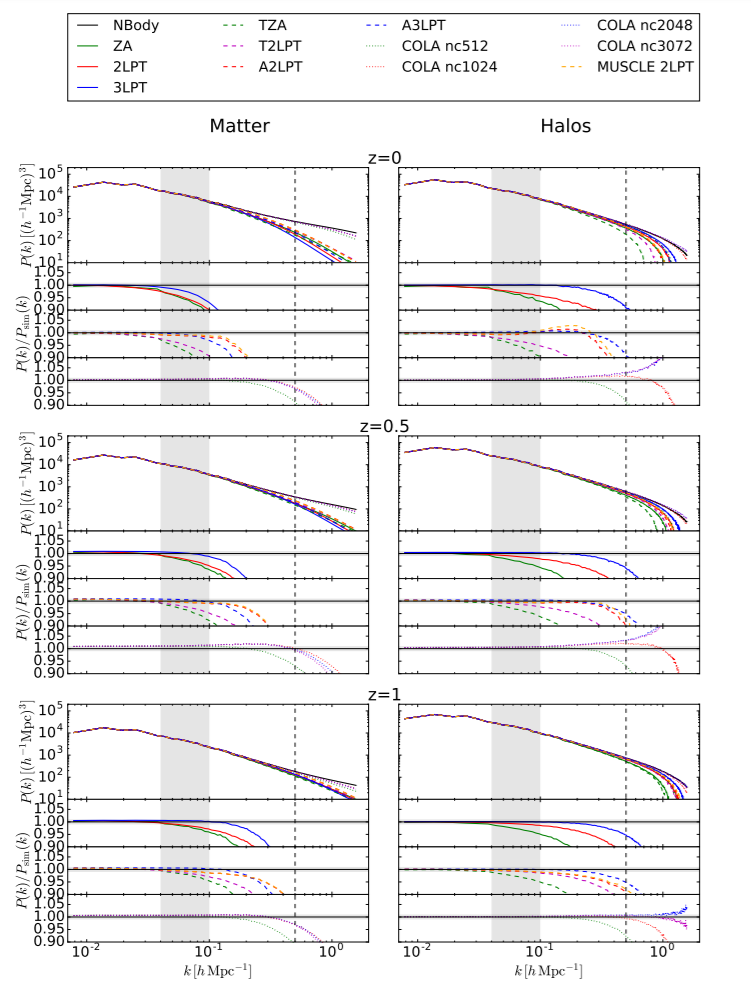
\includegraphics[width=0.9\textwidth]{cosmo_evol/app_compare.png}
    \caption{Power spectrum at $z = 0,\ 0.5$, and $1$ (top, middle, and bottom panels, respectively) in real space and ratio with the \nbody’s one for the matter field (left panels) and the halo catalogs (right panels). The vertical dashed line locates the $k = 0.5\hMpc$ where the one-halo term becomes significant. The vertical shaded area locates the region of the BAO peak, while the horizontal one locates the 1\% accuracy region.  \textit{Note:} Reprinted from \textcite{2017JCAP...07..050M}.}
    \label{fig:app_compare}
\end{figure}